\chapter{Pre-Lab Task}

\section{LTspice Simulation}

We have simulated the Wheatstone Bridge circuit in LTspice. The circuit is shown in Figure \ref{fig:ltspice}. The simulation results are shown in Table \ref{table:ltspice-results}. The simulation results show that the output voltage is zero when the bridge is balanced. The output voltage increases as the bridge becomes unbalanced.

\begin{figure}[h]
    \centering
    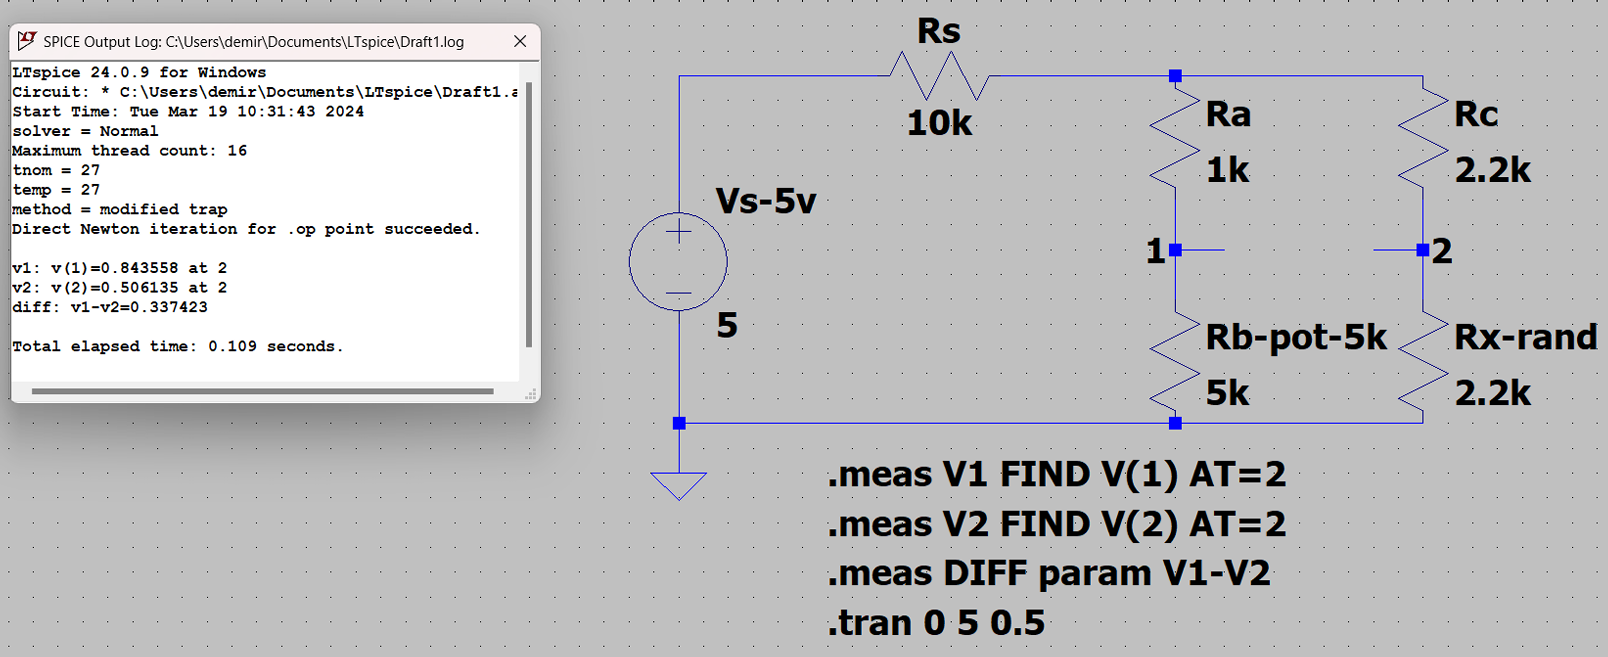
\includegraphics[width=0.7\textwidth]{assets/ltspice.png}
    \caption{LTspice simulation of the Wheatstone Bridge}
    \label{fig:ltspice}
\end{figure}

\begin{table}[h]
    \centering
    \begin{tabular}{|
        >{\columncolor[HTML]{FFCCC9}}l 
        >{\columncolor[HTML]{FFCCC9}}l |
        >{\columncolor[HTML]{FFFC9E}}l 
        >{\columncolor[HTML]{FFFC9E}}l |}
        \hline
        \multicolumn{2}{|l|}{\cellcolor[HTML]{FD6864}For $R_x$ = 2.2k}                      & \multicolumn{2}{l|}{\cellcolor[HTML]{FFCC67}For $R_x$ = 1k}                        \\ \hline
        \multicolumn{1}{|l|}{\cellcolor[HTML]{FD6864}$R_b$} & \cellcolor[HTML]{FD6864}$V_{12}$ & \multicolumn{1}{l|}{\cellcolor[HTML]{FFCC67}$R_b$} & \cellcolor[HTML]{FFCC67}$V_{12}$ \\ \hline
        \multicolumn{1}{|l|}{\cellcolor[HTML]{FFCCC9}1k}   & 0                             & \multicolumn{1}{l|}{\cellcolor[HTML]{FFFC9E}1k}   & 0.10274                       \\ \hline
        \multicolumn{1}{|l|}{\cellcolor[HTML]{FFCCC9}2.2k} & 0.146536                      & \multicolumn{1}{l|}{\cellcolor[HTML]{FFFC9E}2.2k} & 0.258621                      \\ \hline
        \multicolumn{1}{|l|}{\cellcolor[HTML]{FFCCC9}3k}   & 0.216535                      & \multicolumn{1}{l|}{\cellcolor[HTML]{FFFC9E}3k}   & 0.330189                      \\ \hline
        \multicolumn{1}{|l|}{\cellcolor[HTML]{FFCCC9}4k}   & 0.284483                      & \multicolumn{1}{l|}{\cellcolor[HTML]{FFFC9E}4k}   & 0.397959                      \\ \hline
        \multicolumn{1}{|l|}{\cellcolor[HTML]{FFCCC9}5k}   & 0.337423                      & \multicolumn{1}{l|}{\cellcolor[HTML]{FFFC9E}5k}   & 0.44964                       \\ \hline
        \end{tabular}
    \caption{LTspice simulation results of the Wheatstone Bridge circuit}
    \label{table:ltspice-results}
\end{table}

\newpage
\thispagestyle{plain}

\section{Theoretical Analysis}

\begin{figure}[h]
    \centering
    \begin{circuitikz} \draw
        (0,4) to [battery, l=$V_{in}$] (0,0)
        (0,4) -- (4,4)
        node[label={[font=\footnotesize]right:A}] {}
        (4,4) to [R, l=$R_1$] (2,2)
        node[label={[font=\footnotesize]left:C}] {}
        (2,2) to [R, l=$R_2$] (4,0)
        node[label={[font=\footnotesize]right:B}] {}
        (4,0) to [R, l=$R_x$] (6,2)
        node[label={[font=\footnotesize]right:D}] {}
        (6,2) to [vR, l=$R_3$] (4,4)
        (4,0) -- (0,0)
        ;
    \end{circuitikz}
    \caption{Wheatstone Bridge circuit}
    \label{fig:wheatstone-bridge}
\end{figure}

Let's try to derive Wheatstone balance equation to find $R_x$:

\begin{align*}
    V_{out} = V_C - V_D &= V_{R_2} - V_{R_x} = 0 \\
    R_C = \frac{R_2}{R_1+R_2} \quad &\text{and} \quad R_D = \frac{R_x}{R_3+R_x} \\
    \text{At balance,} \quad R_C &= R_D \\
    \frac{R_2}{R_1+R_2} &= \frac{R_x}{R_3+R_x} \\
    R_2(R_3+R_x) &= R_x(R_1+R_2) \\
    R_2R_3 + R_2R_x &= R_x R_1 + R_x R_2 \\
    R_2R_3 &= R_xR_1 \\
    R_x &= \boxed{\frac{R_2R_3}{R_1}}
\end{align*}

\newpage
\thispagestyle{plain}

\section{Numerical Verification}

If we try to verify the Wheatstone balance equation, we can create the following circuit diagram according to the results on the LTspice result table \ref{table:ltspice-results}:

\begin{figure}[h]
    \centering
    \begin{circuitikz} \draw
        (0,4) to [battery, l=$V_{in}$] (0,0)
        (0,4) -- (4,4)
        node[label={[font=\footnotesize]right:A}] {}
        (4,4) to [R, l=1k] (2,2)
        node[label={[font=\footnotesize]left:C}] {}
        (2,2) to [R, l=1k] (4,0)
        node[label={[font=\footnotesize]right:B}] {}
        (4,0) to [R, l=$R_x$] (6,2)
        node[label={[font=\footnotesize]right:D}] {}
        (6,2) to [vR, l=2.2k] (4,4)
        (4,0) -- (0,0)
        ;
    \end{circuitikz}
    \caption{Wheatstone Bridge circuit}
    \label{fig:wheatstone-bridge}
\end{figure}

If we apply the balance equation (Where $V_{CD} = 0$) we can find the value of $R_x$ which should be $2.2k$ according to LTspice result:

\begin{align*}
    R_x &= \frac{R_2R_3}{R_1} \\
    R_x &= \frac{1k \times 2.2k}{1k} \\
    R_x &= 2.2k
\end{align*}

The experimental results are consistent with the theoretical results.
